\documentclass[
  oneside,
  degree=bachelor,
  fullwidthstop=false,
  fontset=fandol,
  times=false,
  minted=false,
  biblatex=true,
]{tongjithesis}

\tjbibresource{bib/ref.bib}

\begin{document}

\renewcommand{\tjheadertext}{课程设计报告}

% ============================================================
%  封面信息
% ============================================================
\school{国豪书院}
\major{计算机科学与技术}
\student{2452627}{徐佳涛}
\thesistitle{手写数字识别与垃圾分类}{——基于 LeNet5 的深度学习课程设计}
\thesistitleeng{Handwritten Digit Recognition and Garbage Classification}{---A LeNet5-Based Deep Learning Course Design}
\thesisadvisor{张红云\quad 教授}
\thesisdate{2026}{5}{25}

% ============================================================
%  信息说明页
% ============================================================

\infotype{thesis}

\infoabstract{%
本课程设计围绕手写数字识别与垃圾分类两个任务展开。首先在 MNIST 手写数字数据集上从零训练 LeNet5 并保存预训练权重，再将该权重迁移到 26 类垃圾分类数据集上，完成从零训练、冻结微调、全量微调、LoRA 微调和强数据增强改进实验。垃圾分类图片统一转换为灰度图，缩放到 $32\times32$，按 MNIST 均值和标准差归一化后输入 LeNet5。实验结果显示：LeNet5 在 MNIST 上达到 98.60\% 的测试准确率；垃圾分类从零训练为 3.85\%，冻结微调为 15.38\%，全量微调为 64.23\%，LoRA 微调为 25.38\%，强数据增强实验为 38.85\%。在此基础上，进一步使用 MobileNetV2 进行进阶对照，其中 MindCV 官方预训练 MobileNetV2-1.0 结合 warmup + cosine 全量微调达到 91.15\%。实验说明 MNIST 预训练权重可以作为有效初始化，但 MNIST 与垃圾分类差异较大，冻结主干适应能力有限；若追求实际准确率，保留 RGB 信息、更高输入分辨率和高质量预训练权重非常关键。
}

\infothesiswords{9000}

\infomaterials{
  \item 项目源代码（LeNet5、LoRA、数据加载、训练评估与曲线绘制模块）；
  \item 实验日志与结果文件（CSV 格式训练日志、JSON 格式结果汇总）；
  \item 训练曲线图和模板版课程设计报告 PDF。
}

\MakeCover
\cleardoublepage
\tjbindinglinefalse

\frontmatter
\MakeAbstract{
    本课程设计围绕《深度学习模块：手写数字识别与垃圾分类》的要求展开。实验首先使用 MindSpore 在 MNIST 手写数字数据集上从零训练 LeNet5，并保存预训练权重；随后将该权重加载到 26 类垃圾分类数据集上，完成从零训练、冻结微调、全量微调、LoRA 微调和模型改进实验。垃圾分类图片在输入 LeNet5 前统一进行 RGB 转灰度、resize 到 $32\times32$、归一化和 HWC 到 CHW 的格式转换。在完成基础迁移实验后，本文进一步使用 MobileNetV2 进行进阶对照，分析更强骨干网络、RGB 输入、高分辨率和 ImageNet 预训练权重对垃圾分类性能的影响。

    实验代码包含数据加载、LeNet5 模型定义、预训练权重加载、冻结策略控制、LoRA 低秩适配、训练评估、CSV 日志记录、JSON 结果汇总和 PNG 曲线绘制等模块。冻结微调中冻结 \texttt{conv1}、\texttt{conv2}、\texttt{fc1}、\texttt{fc2}，只训练最后分类层 \texttt{fc3}；全量微调中所有层参与训练；LoRA 微调中在 \texttt{fc1} 和 \texttt{fc2} 上加入低秩分支，冻结原始主干权重，只训练 LoRA 参数和 \texttt{fc3}。

    实验结果表明：LeNet5 在 MNIST 上达到 98.60\% 的测试准确率；迁移到垃圾分类任务后，从零训练准确率为 3.85\%，冻结微调为 15.38\%，全量微调为 64.23\%，LoRA 微调为 25.38\%，强数据增强改进实验为 38.85\%。结果说明 MNIST 预训练权重可以作为有效初始化，但由于 MNIST 与垃圾分类图像分布差异较大，仅训练最后分类层的冻结微调适应能力不足；全量微调能够重新调整卷积层和全连接层，在 LeNet5 设置下取得最好效果。为进一步考察真实垃圾分类任务的性能上限，本文在正文中加入 MobileNetV2 进阶对照实验：MindCV 官方预训练 MobileNetV2-1.0 结合 warmup + cosine 全量微调达到 91.15\%，说明 RGB 输入、高分辨率和高质量 ImageNet 预训练对真实垃圾分类任务具有显著价值。
}{LeNet5；MNIST；垃圾分类；MindSpore；微调；LoRA}


\clearpage
\tableofcontents
\cleardoublepage

\mainmatter
\chapter{绪论}\label{chap:intro}

\section{实验背景}

LeNet5 与 MNIST 手写数字识别是深度学习图像分类任务中的经典入门组合。LeNet5 通过卷积层提取局部特征，通过池化降低空间分辨率，再利用全连接层完成分类，完整体现了卷积神经网络的基本思想。由于结构清晰、参数量较小、训练流程容易复现，LeNet5 常被用于帮助初学者理解卷积、非线性激活、池化、反向传播和分类损失等基础概念。

课程实验要求在此基础上扩展到 26 类垃圾分类任务。垃圾分类图片来自真实场景，相比 MNIST 具有背景复杂、类别数量更多、类间差异细微等特点。若直接从零训练，模型容易受数据规模限制而学习困难；因此实验采用迁移学习思想，先在 MNIST 上训练 LeNet5，再将预训练权重迁移到垃圾分类数据集上进行微调。

课程资料中以 MobileNetV2 + 垃圾分类作为微调示例，同时也强调 LeNet5 + MNIST 是深度学习入门的核心案例。因此本文采用由浅入深的实验安排：首先使用 LeNet5 完成 MNIST 预训练和垃圾分类迁移，借助较小网络清晰观察层冻结、全量微调和 LoRA 插入机制；随后使用 MobileNetV2 进行进阶对照，分析 RGB 输入、更高分辨率和 ImageNet 预训练权重对真实垃圾分类任务的提升作用。这样的安排既覆盖课程基础要求，也能够进一步讨论实际分类性能的上限。

\section{实验目的}

本课程设计的目标包括：

\begin{enumerate}[label=(\arabic*)]
  \item 使用 MindSpore 实现 LeNet5，并在 MNIST 上完成从零训练，保存预训练权重；
  \item 将 MNIST 预训练权重加载到 26 类垃圾分类任务，完成冻结微调和全量微调；
  \item 在 LeNet5 的 \texttt{fc1} 和 \texttt{fc2} 上加入 LoRA，完成参数高效微调；
  \item 设计垃圾分类从零训练实验，作为无预训练对照；
  \item 设计模型改进实验，在保持超参数一致的前提下仅改变数据增强策略，并比较准确率；
  \item 记录训练时间、显存占用、可训练参数量和验证准确率，形成可复现实验表格；
  \item 引入 MobileNetV2 进阶对照实验，分析更强骨干网络和高质量预训练权重对垃圾分类性能的影响。
\end{enumerate}

\section{本文主要工作}

本文主要完成以下工作：

\begin{enumerate}[label=(\arabic*)]
  \item 使用 MindSpore 实现 LeNet5，并采用具名层结构，便于精确冻结 \texttt{conv1}、\texttt{conv2}、\texttt{fc1}、\texttt{fc2}，并在 \texttt{fc1}、\texttt{fc2} 上插入 LoRA；
  \item 实现垃圾分类图片到 LeNet5 输入的适配流程：RGB 转灰度、resize 到 $32\times32$、归一化、HWC 转 CHW；
  \item 完成 LeNet5 六组实验：MNIST 从零训练、垃圾分类从零训练、冻结微调、全量微调、LoRA 微调和强数据增强改进实验；
  \item 完成 MobileNetV2 进阶实验，对比自实现模型与 MindCV 官方预训练模型在冻结、全量、LoRA 和学习率调度下的表现；
  \item 统一保存 CSV 训练日志、JSON 实验摘要、checkpoint 和 PNG 训练曲线；
  \item 按同济模板组织课程设计报告，并在报告中给出实验原理、代码实现、算法流程和结果分析。
\end{enumerate}

\chapter{实验环境与数据集}\label{chap:env}

\section{实验环境}

实验使用 MindSpore 深度学习框架，项目提供 Docker 配置，推荐在 Windows + Docker Desktop + WSL2 + NVIDIA GPU 环境下运行。容器通过 \texttt{docker compose} 管理，工作目录挂载到容器内的 \texttt{/workspace}，训练生成的 checkpoint、CSV 日志、JSON 摘要和 PNG 曲线会同步保存在本地项目目录。

核心环境验证命令如下：

\begin{lstlisting}[language=bash,numbers=none]
docker compose build
docker compose run --rm mindspore-gpu python -c "import mindspore; mindspore.run_check()"
\end{lstlisting}

如果需要确认 Docker 能够访问 GPU，可使用 NVIDIA CUDA 基础镜像运行 \texttt{nvidia-smi}：

\begin{lstlisting}[language=bash,numbers=none]
docker run --rm --gpus all nvidia/cuda:12.2.0-base-ubuntu22.04 nvidia-smi
\end{lstlisting}

\section{MNIST 数据集}

MNIST 数据集包含 60000 张训练图片和 10000 张测试图片，类别为数字 0 到 9。原始图片为 $28\times28$ 单通道灰度图。为了适配 LeNet5 经典输入尺寸，实验将其 resize 到 $32\times32$，再使用 MNIST 均值 0.1307 和标准差 0.3081 归一化。

\section{垃圾分类数据集}

垃圾分类数据集包含 26 类生活垃圾图片，采用官方 train/test 划分。当前项目中训练集 2593 张，测试/验证集 260 张。类别包括 Banana Peel、Basketball、Battery、Broom、Cans、Cardboard、Ceramic Bowl、Dirty Cloth、Disposable Chopsticks、Eggshell、Fluorescent lamp、Glass Bottle、Glassware、Hats、Lighter、Metalware、Newspaper、Old Mirror、Orange Peel、Paint bucket、Paper、Plastic Bottle、Seashell、Tablet capsules、Toothbrush、Vegetable Leaf。

数据目录结构如下：

\begin{lstlisting}[language=bash,numbers=none]
data/garbage_official/
+-- train/
|   +-- Banana Peel/
|   +-- Basketball/
|   +-- ...
+-- test/
    +-- Banana Peel/
    +-- Basketball/
    +-- ...
\end{lstlisting}

\section{垃圾图片适配 LeNet5}

LeNet5 原始设计面向 $32\times32$ 单通道图像，而垃圾分类数据是 RGB 彩色真实图片。为了加载 MNIST 预训练权重并保持输入形式一致，本文采用如下预处理：

\begin{enumerate}[label=(\arabic*)]
  \item 使用 PIL 读取图片并转换为灰度图；
  \item 将图片 resize 到 $32\times32$；
  \item 将像素缩放到 $[0,1]$；
  \item 使用 MNIST 均值和标准差归一化；
  \item 将图像从 HWC 格式转换为 MindSpore 常用的 CHW 格式。
\end{enumerate}

该流程使垃圾分类图片能够直接输入 LeNet5，但也带来三个局限：灰度化会丢失颜色信息；$32\times32$ 输入会损失真实物体细节；LeNet5 模型容量较小，对 26 类真实场景分类的表达能力有限。

\chapter{模型原理与微调方法}\label{chap:theory}

\section{LeNet5 网络结构}

LeNet5 是早期经典卷积神经网络，由 LeCun 等人在手写数字识别研究中提出\cite{lenet1998}。本文实现的 LeNet5 由两个卷积层、两个池化层和三个全连接层组成，输入为单通道 $32\times32$ 图像。结构如下：

\[
\text{Conv1}(1,6,5) \rightarrow \text{ReLU} \rightarrow \text{MaxPool}
\rightarrow \text{Conv2}(6,16,5) \rightarrow \text{ReLU} \rightarrow \text{MaxPool}
\rightarrow \text{FC1}(400,120) \rightarrow \text{FC2}(120,84) \rightarrow \text{FC3}(84,C)
\]

其中 $C$ 为类别数，在 MNIST 任务中为 10，在垃圾分类任务中为 26。卷积层负责提取局部边缘与纹理，池化层降低空间分辨率并增强局部不变性，全连接层完成高层特征组合和分类。

\section{MNIST 预训练}

MNIST 预训练阶段使用 10 类手写数字数据训练 LeNet5，得到 \texttt{checkpoints/lenet\_mnist.ckpt}。代码基于 MindSpore 框架实现\cite{mindspore}。该权重包含卷积层和前两个全连接层学到的基础图像特征。迁移到垃圾分类时，最后分类层输出维度从 10 改为 26，因此 \texttt{fc3} 无法直接加载 MNIST 权重，需要重新初始化并训练。

为了兼容旧版本 SequentialCell 保存的 checkpoint，代码中提供了参数名映射，将旧参数名如 \texttt{net.0.weight}、\texttt{net.7.weight} 映射到新具名层 \texttt{conv1.weight}、\texttt{fc1.weight} 等。

\section{冻结微调}

冻结微调加载 MNIST 预训练权重后，冻结 \texttt{conv1}、\texttt{conv2}、\texttt{fc1}、\texttt{fc2}，只训练最后分类层 \texttt{fc3}。该策略的优点是可训练参数量少、显存占用低、训练过程稳定；缺点是模型只能在线性分类头上适配新任务，当源任务和目标任务差异较大时，上限较低。

本实验中，冻结微调的可训练参数为 \texttt{fc3.weight} 和 \texttt{fc3.bias}，共 2210 个参数。

\section{全量微调}

全量微调同样加载 MNIST 预训练权重，但所有层都参与训练。这样模型可以根据垃圾分类数据重新调整低层卷积特征和高层全连接特征，适配能力最强。其代价是可训练参数量、显存和过拟合风险更高。由于 LeNet5 总参数量仅约 6.3 万，本实验中全量微调仍然具有较低计算成本。

\section{LoRA 微调}

LoRA（Low-Rank Adaptation）的核心思想是冻结原始权重 $W$，只学习一个低秩更新\cite{lora2022}：

\[
W'x = Wx + BAx \cdot \frac{\alpha}{r}
\]

其中 $A$ 将输入特征降到秩 $r$，$B$ 将低维特征映射回输出维度，$\alpha/r$ 为缩放系数。训练开始时通常将 $B$ 初始化为零，使 LoRA 分支初始输出为零，从而不破坏预训练模型的行为。

本文将 LoRA 加在 LeNet5 的 \texttt{fc1} 和 \texttt{fc2} 上，冻结原始 \texttt{conv1}、\texttt{conv2}、\texttt{fc1}、\texttt{fc2} 主分支，只训练 \texttt{fc1/fc2} 的 LoRA 参数和最后分类层 \texttt{fc3}。需要说明的是，LeNet5 总参数量只有约 6.3 万，本身已经是轻量模型，因此 LoRA 在本实验中的主要价值不是节省工业级大模型的显存和吞吐成本，而是验证在 MindSpore 中手动插入低秩适配器、冻结主干并只训练增量分支的可行性。

\section{模型改进实验}

模型改进实验采用更强数据增强：在全量微调基础上增加随机旋转和随机水平翻转。为保证公平对比，增强实验与全量微调基线保持相同的 epoch、batch size、学习率、权重衰减、输入尺寸和随机种子，仅改变 \texttt{--strong\_aug} 这一项。由于增强实验结果明显下降，后续分析将其作为一次负向消融，并结合预处理可视化检查增强配置是否引入了不合理伪特征。

\section{MobileNetV2 进阶对照模型原理}

课程资料中也以 MobileNetV2 + 垃圾分类作为微调示例。为了进一步比较经典小型 CNN 与现代轻量级 CNN 在垃圾分类上的差异，本文在 LeNet5 实验之外加入 MobileNetV2 进阶对照实验。MobileNetV2 是 Google 提出的轻量级卷积网络\cite{mobilenetv2}，核心结构包括深度可分离卷积、倒残差连接和线性瓶颈。

标准卷积同时在空间维度和通道维度上进行卷积，计算量较大。深度可分离卷积将其拆分为 depthwise convolution 和 pointwise convolution：前者对每个通道独立进行空间卷积，后者使用 $1\times1$ 卷积融合通道信息。这样可以显著减少参数量和计算量。

MobileNetV2 的倒残差模块通常包含三步：

\begin{enumerate}[label=(\arabic*)]
  \item 使用 $1\times1$ pointwise convolution 扩展通道数；
  \item 使用 $3\times3$ depthwise convolution 提取空间特征；
  \item 使用 $1\times1$ pointwise convolution 将通道数压回较低维度，并在瓶颈处保持线性输出。
\end{enumerate}

倒残差结构与传统残差结构的差别在于：传统残差网络通常先降维、再卷积、最后升维，而 MobileNetV2 先升维到更高通道空间中提取特征，再压缩回低维瓶颈。这样做可以让非线性激活主要发生在高维空间，减少低维瓶颈中信息被 ReLU 截断的风险。线性瓶颈则避免在最后压缩阶段继续使用非线性激活，从而更好地保存类别判别所需的信息。

在垃圾分类任务中，MobileNetV2 的优势主要体现在两方面。其一，RGB 输入和 $224\times224$ 分辨率能保留颜色、材质、反光、纹理和边缘细节，这些信息对塑料、金属、纸张、玻璃、厨余等类别区分非常重要。其二，ImageNet 预训练权重来自大规模自然图像分类任务，已经学习到通用视觉特征，因此在小规模垃圾分类数据集上只需较少样本即可完成迁移。

与 LeNet5 相比，MobileNetV2 使用 RGB 输入和 $224\times224$ 分辨率，能够保留颜色、纹理和局部细节；同时 ImageNet 预训练权重提供了边缘、纹理、形状乃至语义层面的通用视觉特征。因此 MobileNetV2 进阶对照实验主要用于验证更强骨干网络和高质量预训练初始化对垃圾分类准确率上限的影响。

\chapter{代码实现与算法流程}\label{chap:design}

\section{项目模块}

基础实验与对照实验代码主要由以下文件组成：

\begin{itemize}
  \item \texttt{src/model.py}：定义 LeNet5、MobileNetV2 和 SmallCNN。LeNet5 使用具名层，并支持 Dropout 和 FC 层 LoRA；
  \item \texttt{src/lora.py}：定义 LoRAConv2d、LoRADense 和 LoRADenseFromBase；
  \item \texttt{src/train\_mnist\_lenet.py}：在 MNIST 上从零训练 LeNet5 并保存预训练权重；
  \item \texttt{src/train\_lenet\_garbage.py}：完成垃圾分类从零训练、冻结微调、全量微调、LoRA 微调和增强实验；
  \item \texttt{src/eval\_lenet.py}：加载 LeNet5 checkpoint 并在垃圾分类验证集上评估；
  \item \texttt{src/plot\_curves.py}：读取 CSV 训练日志并绘制损失和准确率曲线；
  \item \texttt{src/utils.py}：提供随机种子、显存统计、CSV/JSON 写入和参数统计工具；
  \item \texttt{scripts/run\_lenet\_experiments.ps1}：一键运行全部 LeNet5 实验。
\end{itemize}

\section{LeNet5 实现}

为了精确控制层冻结、参数统计和 LoRA 插入，本文将 LeNet5 写成具名层结构：

\begin{lstlisting}[language=Python,numbers=none]
self.conv1 = nn.Conv2d(1, 6, kernel_size=5, pad_mode="valid")
self.conv2 = nn.Conv2d(6, 16, kernel_size=5, pad_mode="valid")
self.fc1 = nn.Dense(16 * 5 * 5, 120)
self.fc2 = nn.Dense(120, 84)
self.fc3 = nn.Dense(84, num_classes)
\end{lstlisting}

当 \texttt{use\_lora=True} 时，\texttt{fc1} 和 \texttt{fc2} 会被 LoRADenseFromBase 包装。原始 Dense 权重作为冻结主分支，LoRA 分支作为可训练低秩更新。

\section{训练模式控制}

垃圾分类脚本通过 \texttt{--mode} 参数控制训练策略：

\begin{lstlisting}[language=bash,numbers=none]
--mode scratch  # 不加载 MNIST 权重，全部参数训练
--mode freeze   # 加载 MNIST 权重，只训练 fc3
--mode full     # 加载 MNIST 权重，全部参数训练
--mode lora     # 加载 MNIST 权重，训练 fc1/fc2 LoRA 和 fc3
\end{lstlisting}

冻结策略由参数名控制。冻结微调中仅 \texttt{fc3.weight} 和 \texttt{fc3.bias} 的 \texttt{requires\_grad=True}。LoRA 微调中，名称包含 \texttt{lora\_} 的参数以及 \texttt{fc3} 参数参与训练。

\section{训练日志与结果保存}

每个 epoch 结束后，脚本会向 CSV 写入以下字段：epoch、训练损失、训练准确率、验证准确率、epoch 用时、GPU 显存、可训练参数量、是否启用强增强和 Dropout 值。训练结束后，JSON summary 保存最优准确率、总训练时间、参数量、冻结策略、LoRA 配置和 best checkpoint 路径。

训练曲线由 \texttt{src/plot\_curves.py} 绘制，包括训练损失曲线以及训练/验证准确率曲线。所有曲线保存为 PNG，便于在报告中引用。

\section{一键实验流程}

一键脚本 \texttt{scripts/run\_lenet\_experiments.ps1} 的算法流程如下：

\begin{enumerate}[label=(\arabic*)]
  \item 训练 LeNet5 + MNIST，保存 \texttt{checkpoints/lenet\_mnist.ckpt}；
  \item 绘制 MNIST 训练曲线；
  \item 在垃圾分类上从零训练 LeNet5；
  \item 加载 MNIST 权重，进行冻结微调；
  \item 加载 MNIST 权重，进行全量微调；
  \item 加载 MNIST 权重，进行 LoRA 微调；
  \item 在全量微调基础上启用强数据增强，完成模型改进实验；
  \item 为五组垃圾分类实验分别绘制训练曲线；
  \item 输出所有 JSON summary，便于填入报告表格。
\end{enumerate}

\chapter{实验结果与分析}\label{chap:experiment}

\section{实验设置}

所有 LeNet5 垃圾分类实验均采用官方 train/test 划分，训练集 2593 张，验证集 260 张。输入图片统一转灰度并 resize 到 $32\times32$。优化器使用 Adam，垃圾分类实验统一训练 24 个 epoch，batch size 为 32，学习率为 $1\times10^{-3}$，权重衰减为 $1\times10^{-4}$。LoRA 实验设置 rank 为 4，alpha 为 8。

\section{MNIST 预训练结果}

LeNet5 在 MNIST 上训练 5 个 epoch，结果如\cref{tab:mnist_result} 所示。测试准确率达到 98.60\%，说明模型实现和训练流程正确，生成的 \texttt{checkpoints/lenet\_mnist.ckpt} 可作为后续垃圾分类微调的初始化。

\begin{table}[!htb]
  \centering
  \caption{LeNet5 在 MNIST 上的预训练结果}
  \label{tab:mnist_result}
  \begin{tabular}{@{}lrrrrr@{}}
    \toprule
    \textbf{实验} & \textbf{训练样本} & \textbf{测试样本} & \textbf{可训练参数} & \textbf{时间} & \textbf{准确率} \\
    \midrule
    LeNet5 + MNIST 从零训练 & 60000 & 10000 & 61684 & 266.77 s & 98.60\% \\
    \bottomrule
  \end{tabular}
\end{table}

\begin{figure}[!htb]
  \centering
  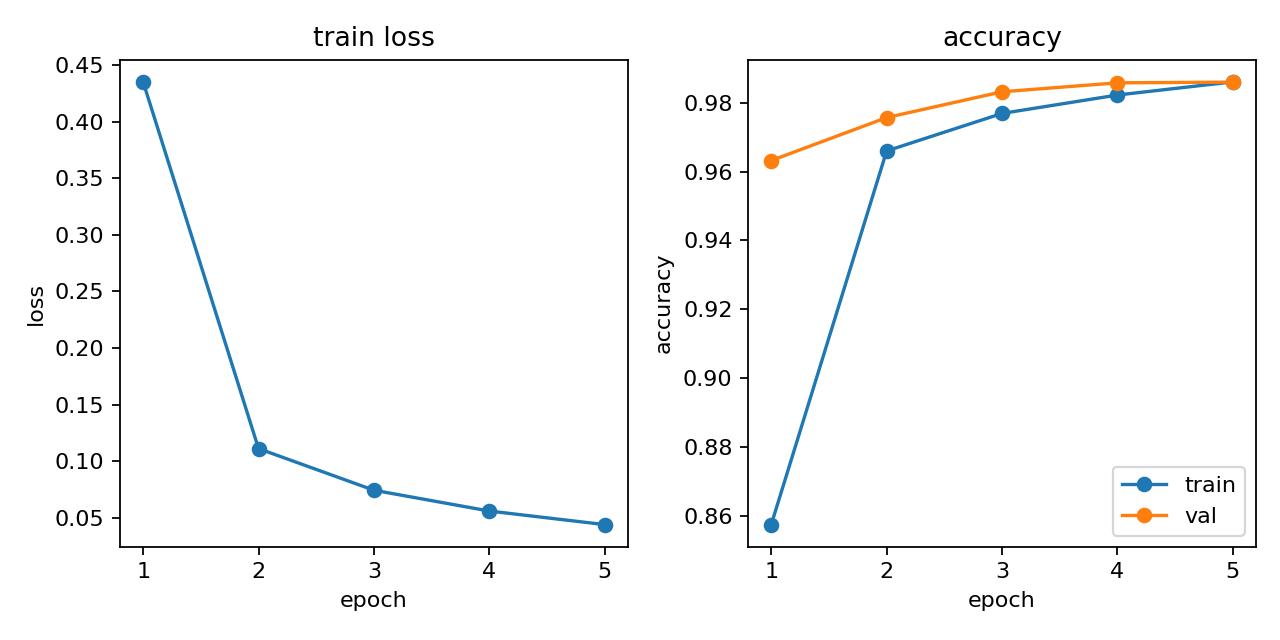
\includegraphics[width=0.86\linewidth]{figures/curve_lenet_mnist.png}
  \caption{LeNet5 在 MNIST 上的训练曲线}
  \label{fig:curve_mnist}
\end{figure}

\section{LeNet5 垃圾分类实验}

垃圾分类四组对比实验结果如\cref{tab:garbage_compare} 所示。

\begin{table}[!htb]
  \centering
  \caption{LeNet5 垃圾分类训练与微调结果}
  \label{tab:garbage_compare}
  \small
  \begin{tabular}{@{}lrrrrr@{}}
    \toprule
    \textbf{实验} & \textbf{可训练参数} & \textbf{总参数} & \textbf{时间} & \textbf{峰值显存} & \textbf{准确率} \\
    \midrule
    从零训练 & 63044 & 63044 & 362.80 s & 3698 MB & 3.85\% \\
    冻结微调 & 2210 & 63044 & 376.04 s & 3610 MB & 15.38\% \\
    全量微调 & 63044 & 63044 & 362.99 s & 3698 MB & 64.23\% \\
    LoRA 微调 & 5106 & 65940 & 379.66 s & 3610 MB & 25.38\% \\
    \bottomrule
  \end{tabular}
\end{table}

从零训练准确率仅为 3.85\%，接近 26 类随机猜测水平，说明小规模垃圾分类数据不足以让 LeNet5 从随机初始化中快速学到稳定特征。冻结微调将准确率提升到 15.38\%，说明 MNIST 预训练权重有一定帮助，但仅训练最后分类层的适应能力仍有限。

全量微调达到 64.23\%，是四组对比实验中最佳结果。原因在于所有卷积层和全连接层都可以根据垃圾分类图片重新调整，能够弥补 MNIST 与垃圾分类之间的分布差异。LoRA 微调的可训练参数为 5106，显存为 3610 MB，准确率为 25.38\%，高于冻结微调但低于全量微调。

需要务实指出的是，LeNet5 总参数量很小，全量微调与 LoRA 微调的峰值显存只相差 88 MB，训练时间也没有减少，LoRA 反而略慢。因此在 LeNet5 这种轻量网络上，LoRA 的实际工程收益很有限。本实验中 LoRA 的意义主要在于验证低秩分支插入、主干冻结和增量参数训练的实现流程，而不是证明 LoRA 在小模型上具有实用性能优势。

\section{训练曲线}

\begin{figure}[!htb]
  \centering
  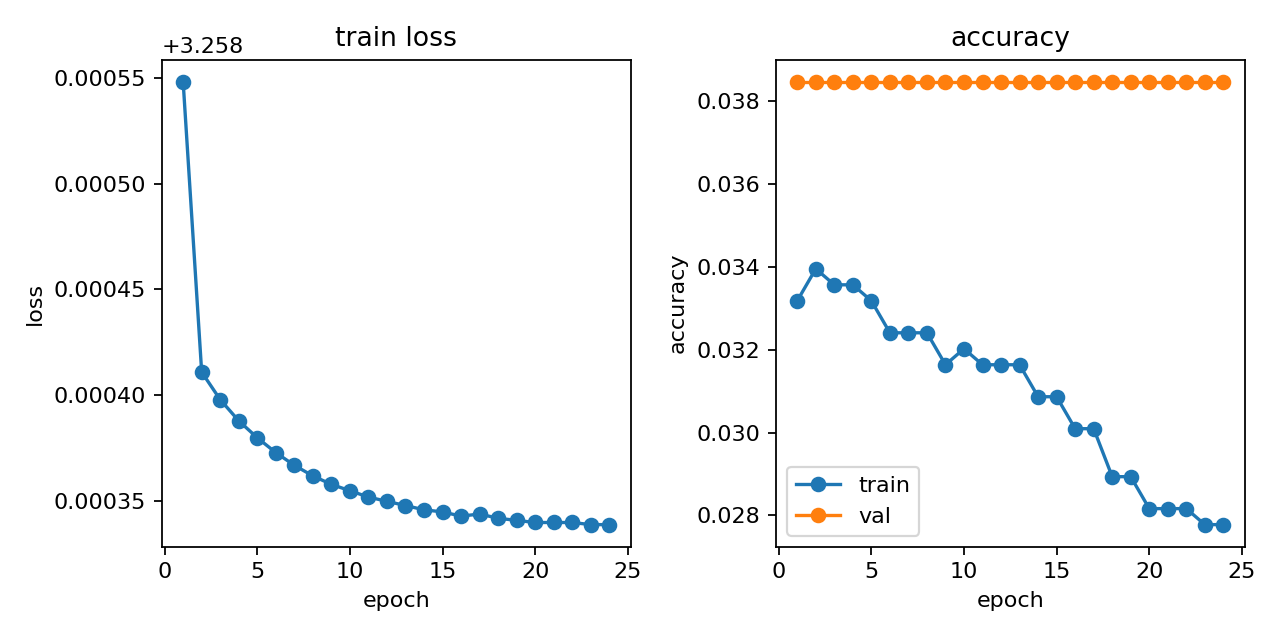
\includegraphics[width=0.82\linewidth]{figures/curve_lenet_garbage_scratch.png}
  \caption{LeNet5 垃圾分类从零训练曲线}
  \label{fig:curve_scratch}
\end{figure}

\begin{figure}[!htb]
  \centering
  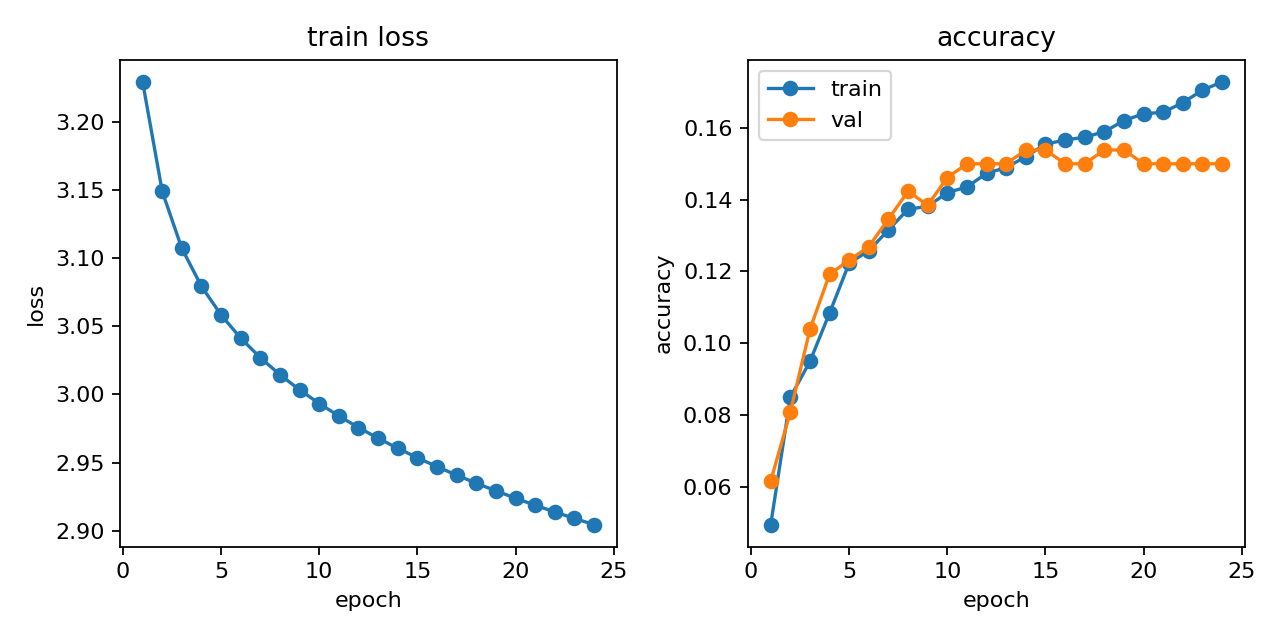
\includegraphics[width=0.82\linewidth]{figures/curve_lenet_garbage_freeze.png}
  \caption{LeNet5 垃圾分类冻结微调曲线}
  \label{fig:curve_freeze}
\end{figure}

\begin{figure}[!htb]
  \centering
  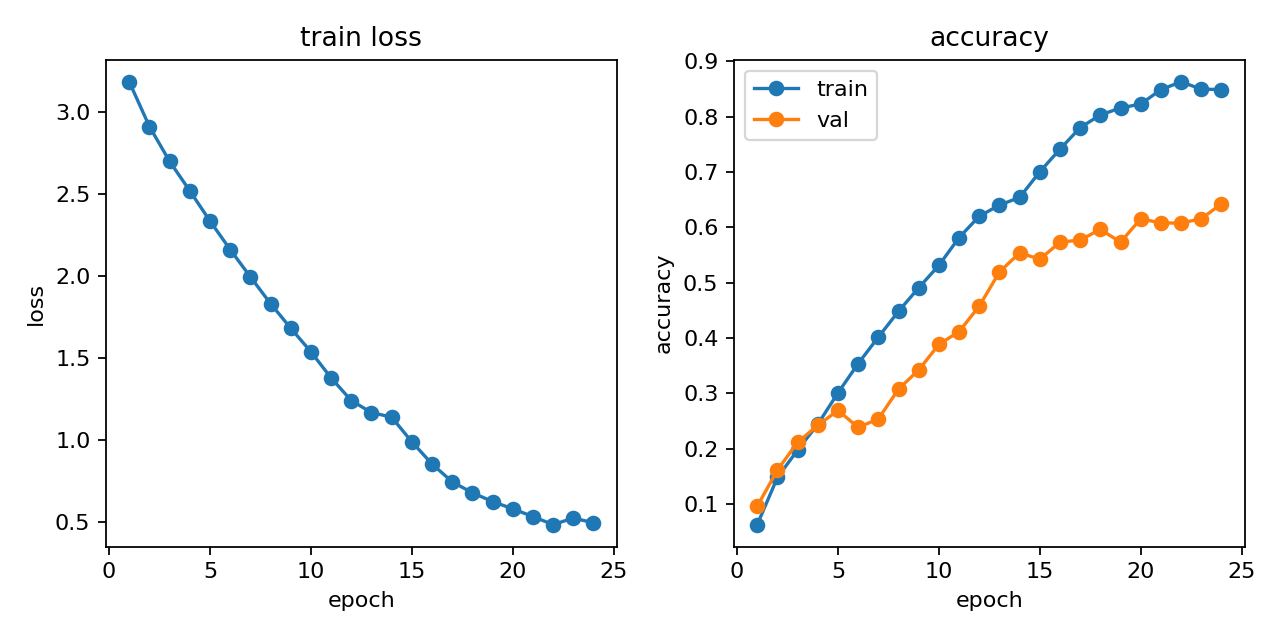
\includegraphics[width=0.82\linewidth]{figures/curve_lenet_garbage_full.png}
  \caption{LeNet5 垃圾分类全量微调曲线}
  \label{fig:curve_full}
\end{figure}

\begin{figure}[!htb]
  \centering
  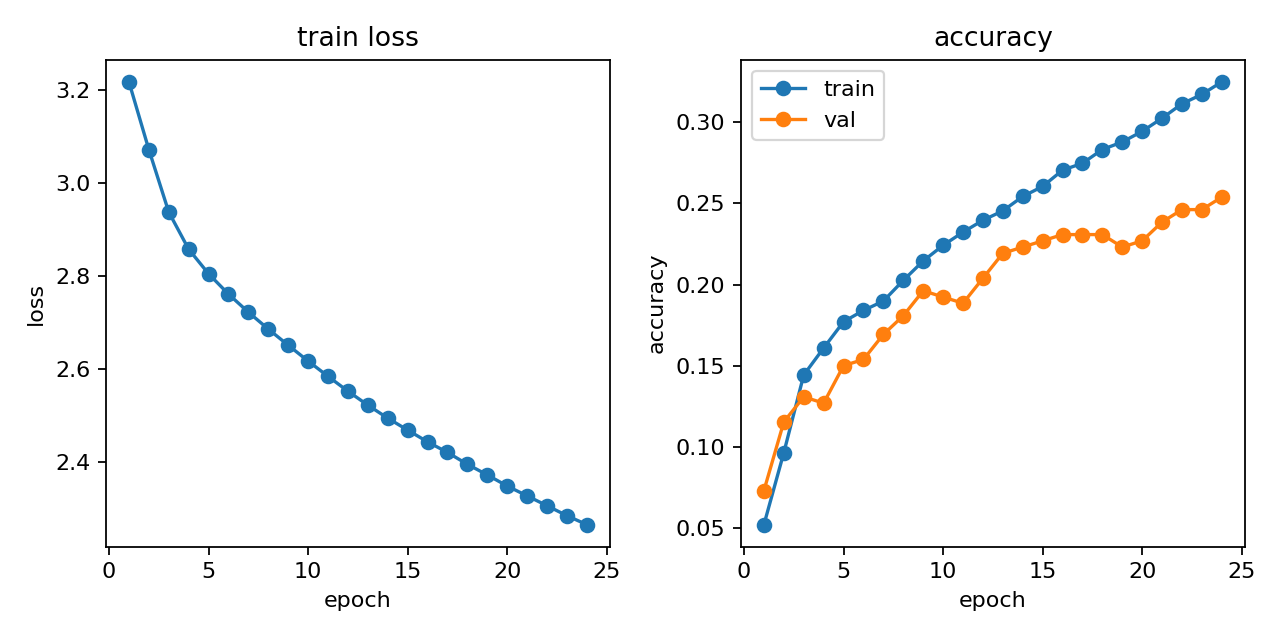
\includegraphics[width=0.82\linewidth]{figures/curve_lenet_garbage_lora.png}
  \caption{LeNet5 垃圾分类 LoRA 微调曲线}
  \label{fig:curve_lora}
\end{figure}

\section{模型改进实验}

模型改进实验在全量微调基础上启用 \texttt{--strong\_aug}，即增加随机旋转和随机水平翻转。除增强项外，epoch、batch size、学习率、权重衰减、输入尺寸和随机种子均保持一致。结果如\cref{tab:aug_compare} 所示。

\begin{table}[!htb]
  \centering
  \caption{强数据增强改进实验}
  \label{tab:aug_compare}
  \begin{tabular}{@{}lrrrr@{}}
    \toprule
    \textbf{实验} & \textbf{改动} & \textbf{可训练参数} & \textbf{时间} & \textbf{准确率} \\
    \midrule
    全量微调基线 & 默认预处理 & 63044 & 362.99 s & 64.23\% \\
    强数据增强 & 随机旋转 + 水平翻转 & 63044 & 364.80 s & 38.85\% \\
    \bottomrule
  \end{tabular}
\end{table}

\begin{figure}[!htb]
  \centering
  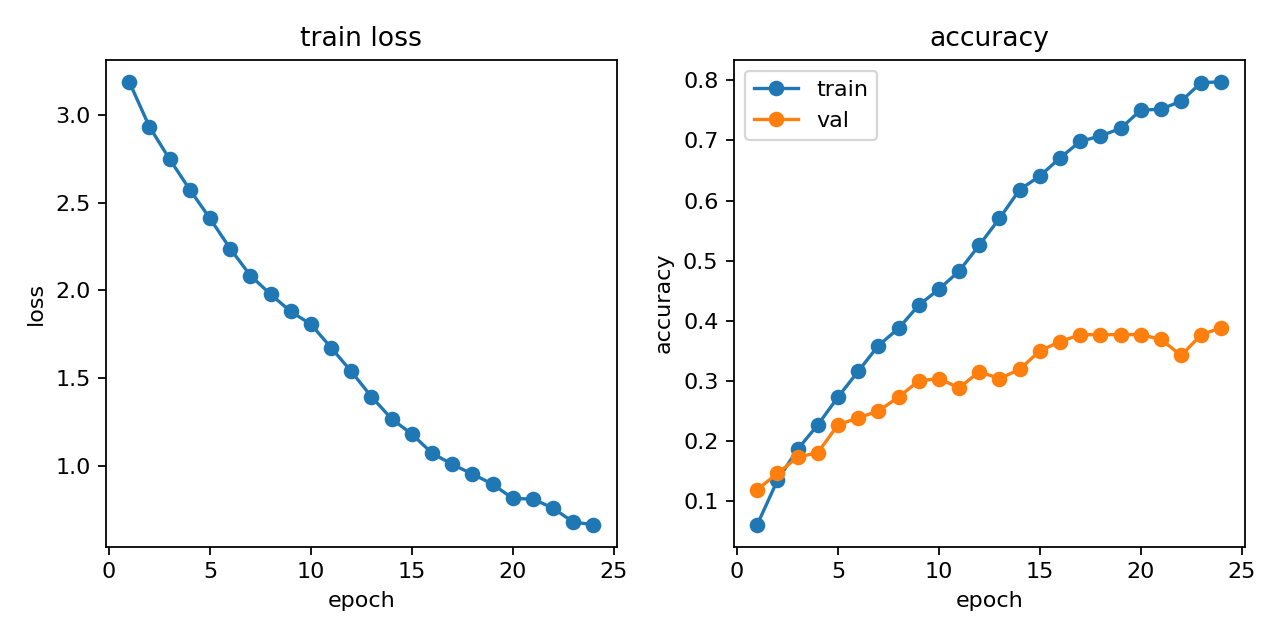
\includegraphics[width=0.82\linewidth]{figures/curve_lenet_garbage_full_aug.png}
  \caption{LeNet5 强数据增强改进实验曲线}
  \label{fig:curve_aug}
\end{figure}

强数据增强没有带来提升，准确率从 64.23\% 降至 38.85\%。这不是一个可以简单解释为“增强不适合垃圾分类”的结果，因为水平翻转和适度旋转通常属于保持标签不变的数据增强。为排查原因，本文额外保存了增强前后的输入可视化，如\cref{fig:preprocess_preview} 所示。

\begin{figure}[!htb]
  \centering
  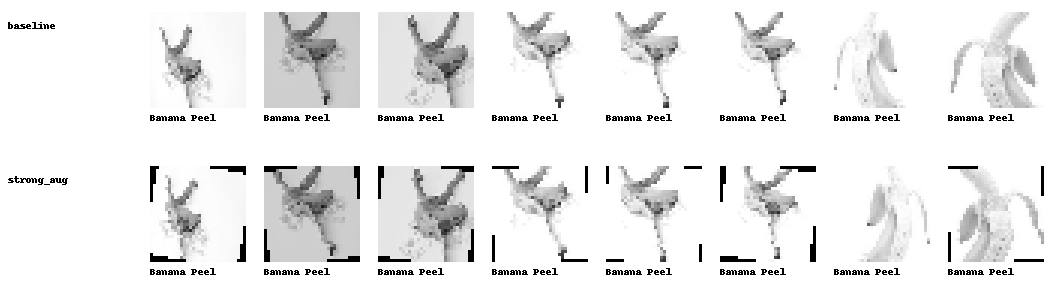
\includegraphics[width=0.92\linewidth]{figures/preprocess_lenet_preview.png}
  \caption{LeNet5 输入预处理可视化：baseline 与 strong\_aug 对比}
  \label{fig:preprocess_preview}
\end{figure}

可视化结果显示，随机旋转后的 $32\times32$ 灰度图出现了明显黑色边框。由于 LeNet5 输入尺寸很小，这些边框在图像中占比较高，可能成为与类别无关的强伪特征，干扰模型学习。更合理的做法是调整旋转填充值、使用中心裁剪/反射填充，或先在更高分辨率下增强再缩放。因此本文将该实验视为一次负向消融：它暴露了增强算子配置与低分辨率输入之间的冲突，而不是说明数据增强思想本身无效。

\section{综合分析}

从准确率看，全量微调明显优于冻结微调和 LoRA 微调，说明当前任务需要更新全部 LeNet5 参数以适配真实垃圾图片。从可训练参数看，冻结微调最省参数，仅 2210 个；LoRA 微调为 5106 个，在显存占用与冻结微调相近的情况下取得更高准确率；全量微调参数最多，但由于 LeNet5 规模较小，训练成本仍可接受。

从显存看，冻结微调和 LoRA 微调峰值显存为 3610 MB，低于全量微调和从零训练的 3698 MB，但差距只有 88 MB。训练时间差异也不大，主要受数据加载和容器开销影响。综合而言，在 LeNet5 这种小模型上，全量微调是准确率最优策略；LoRA 的工程节省并不明显，更适合作为参数高效微调机制的实现验证；冻结微调适合作为低成本基线。

\section{进阶对照实验：MobileNetV2}

LeNet5 实验完成了从 MNIST 预训练到垃圾分类微调的完整链路，适合观察卷积层、全连接层、冻结策略和 LoRA 分支的具体作用。但从真实垃圾分类任务本身看，LeNet5 的输入被压缩为 $32\times32$ 灰度图，模型容量也较小，容易形成性能上限。为进一步回答“如果使用课程资料中更接近实际应用的轻量级网络，垃圾分类可以达到什么水平”，本文加入 MobileNetV2 进阶对照实验。

MobileNetV2 对照实验和 LeNet5 的关键差异有三点。第一，输入保持 RGB 三通道并 resize 到 $224\times224$，能够保留颜色和更丰富的局部纹理；第二，网络由倒残差模块和 depthwise separable convolution 组成，参数量明显高于 LeNet5，但仍属于轻量级 CNN；第三，官方 ImageNet 预训练权重提供了大规模自然图像上的通用视觉特征。通过这组实验，可以判断 LeNet5 结果到底受限于训练流程，还是受限于输入适配和模型表达能力。

MobileNetV2 对照实验分为两条线。第一条线是自实现 MobileNetV2，用于观察在没有完整匹配官方预训练权重时，大模型是否自然优于小模型。第二条线是 MindCV 官方 MobileNetV2，用于观察结构、参数名和预训练 checkpoint 完整匹配时，迁移学习在垃圾分类上的实际表现。

\subsection{自实现 MobileNetV2 基线}

自实现 MobileNetV2 使用 RGB 输入和 $224\times224$ 分辨率，参数量约 229 万。该模型主要由 ConvBNReLU、InvertedResidual 和全局平均池化分类头组成。与 LeNet5 不同，它保留了 RGB 颜色信息，并使用 ImageNet 常用均值和标准差归一化。

未加载完整匹配的官方预训练权重时，三种策略结果如\cref{tab:mobile_self} 所示。

\begin{table}[!htb]
  \centering
  \caption{自实现 MobileNetV2 基线结果}
  \label{tab:mobile_self}
  \small
  \begin{tabular}{@{}lrrrr@{}}
    \toprule
    \textbf{策略} & \textbf{可训练参数} & \textbf{总参数} & \textbf{时间} & \textbf{准确率} \\
    \midrule
    freeze & 33306 & 2291290 & 328.15 s & 17.31\% \\
    full & 2291290 & 2291290 & 544.21 s & 51.92\% \\
    LoRA & 107418 & 2365402 & 550.82 s & 40.38\% \\
    \bottomrule
  \end{tabular}
\end{table}

这组结果说明，更大的网络如果缺少高质量初始化，并不必然优于 LeNet5。自实现 MobileNetV2 全量微调为 51.92\%，低于 LeNet5 全量微调的 64.23\%。其原因主要有两点：一是垃圾分类训练集只有 2593 张，较大模型从随机或不充分预训练状态开始训练时更容易受数据规模限制；二是 MobileNetV2 依赖 BatchNorm、倒残差堆叠和更深层特征传递，如果预训练权重未完整匹配，早期训练阶段的特征分布不稳定。

冻结微调只有 17.31\%，说明未充分预训练的 backbone 不能直接作为特征提取器。此时只训练最后分类头，相当于用一组质量不高且不可更新的特征做线性分类，上限自然很低。LoRA 达到 40.38\%，高于冻结但低于全量，说明在较大网络中低秩分支比只训练分类头更灵活，可以对中后层特征进行一定修正；但在缺少高质量预训练表示时，LoRA 仍然无法完全替代全量参数更新。

因此，自实现 MobileNetV2 的价值不在于取得最高准确率，而在于说明迁移学习不是“模型越大越好”的简单问题。模型结构、预训练权重、参数加载匹配程度和学习率策略必须同时成立，才能发挥现代 CNN 的优势。

\subsection{MindCV 官方预训练 MobileNetV2}

进一步使用 MindCV 官方 MobileNetV2-1.0，并加载匹配的 ImageNet 预训练 checkpoint。与自实现模型相比，官方模型的结构定义、参数命名和 checkpoint 对齐程度更高，能够加载 260 个匹配参数。实验同样比较冻结微调、全量微调和 LoRA 微调，并额外测试了常量学习率与 warmup + cosine 学习率调度的差异。结果如\cref{tab:mobile_mindcv} 所示。

\begin{table}[!htb]
  \centering
  \caption{MindCV 官方预训练 MobileNetV2-1.0 结果}
  \label{tab:mobile_mindcv}
  \small
  \begin{tabular}{@{}lrrrr@{}}
    \toprule
    \textbf{策略} & \textbf{LR 策略} & \textbf{可训练参数} & \textbf{时间} & \textbf{准确率} \\
    \midrule
    freeze & constant & 33306 & 378.99 s & 87.31\% \\
    full & constant & 2291290 & 627.08 s & 8.08\% \\
    full & cosine + warmup & 2291290 & 622.66 s & 91.15\% \\
    LoRA & constant & 80922 & 459.41 s & 89.62\% \\
    \bottomrule
  \end{tabular}
\end{table}

官方预训练 MobileNetV2 的结果显著高于 LeNet5。冻结微调已达到 87.31\%，说明 ImageNet 预训练 backbone 已经具备较强的通用特征提取能力，即使只替换并训练最后分类头，也能较好地区分 26 类垃圾图像。LoRA 微调达到 89.62\%，在只训练约 8.1 万参数的情况下进一步超过冻结微调，说明低秩分支能够在保留主干预训练特征的同时，对垃圾分类的高层语义表示进行轻量修正。全量微调配合 warmup + cosine 学习率衰减达到 91.15\%，是所有实验中最高的结果，说明当优化策略合适时，开放全部参数可以进一步提高模型对目标数据分布的适配能力。

值得注意的是，full constant 只有 8.08\%，远低于 freeze 和 LoRA。这个结果说明预训练模型全量微调不能简单使用固定学习率直接训练。全量开放参数后，反向传播会同时改变低层边缘纹理特征和高层语义特征；如果学习率调度不稳，模型可能在前几个 epoch 快速破坏原有预训练表示，导致验证准确率崩溃。相比之下，warmup + cosine 先用较小步长平稳适配新分类头和中高层特征，再逐步衰减学习率，有利于在“保留通用特征”和“适配新任务”之间取得平衡。

从任务角度看，这组结果还说明垃圾分类图片中颜色和分辨率非常重要。例如塑料、金属、纸张、果皮等类别不仅依赖形状轮廓，也依赖颜色、反光、纹理和局部细节。LeNet5 为了适配 MNIST 预训练链路将图片灰度化并压缩到 $32\times32$，便于完成可解释的迁移学习实验；MobileNetV2 则保留更接近真实视觉任务的输入形态，因此能显著提高准确率。

\begin{figure}[!htb]
  \centering
  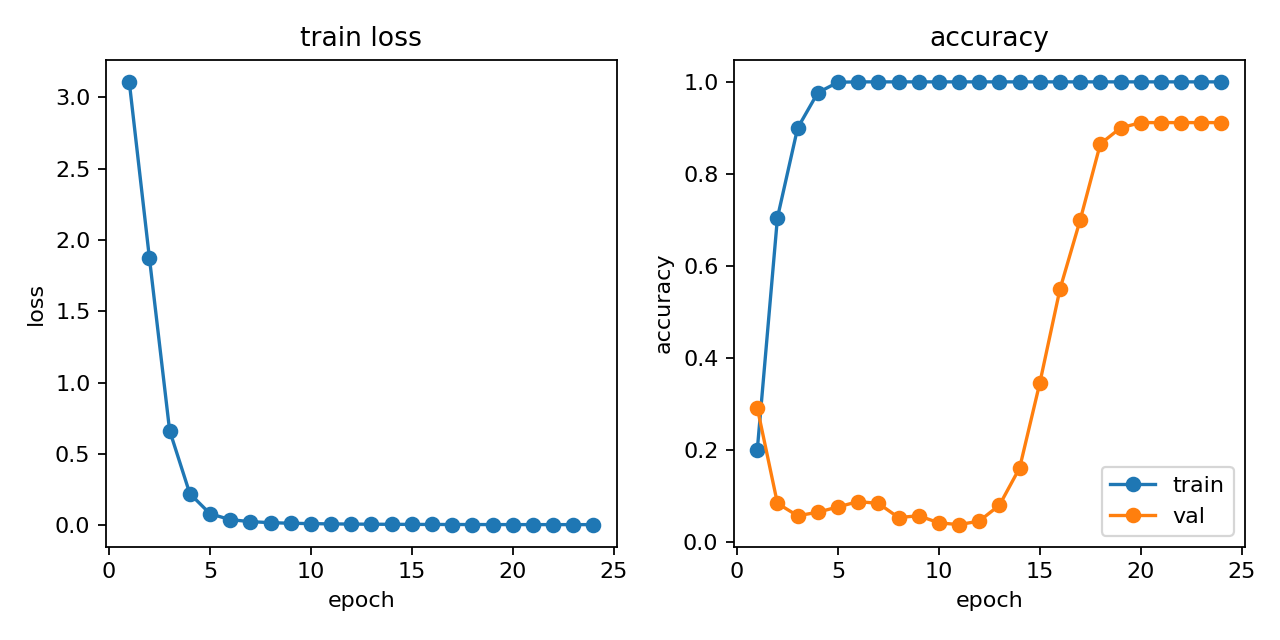
\includegraphics[width=0.82\linewidth]{figures/curve_mindcv_mobilenet_v2_100_full_cosine.png}
  \caption{MindCV MobileNetV2-1.0 full + cosine 训练曲线}
  \label{fig:mobile_full_cosine}
\end{figure}

\begin{figure}[!htb]
  \centering
  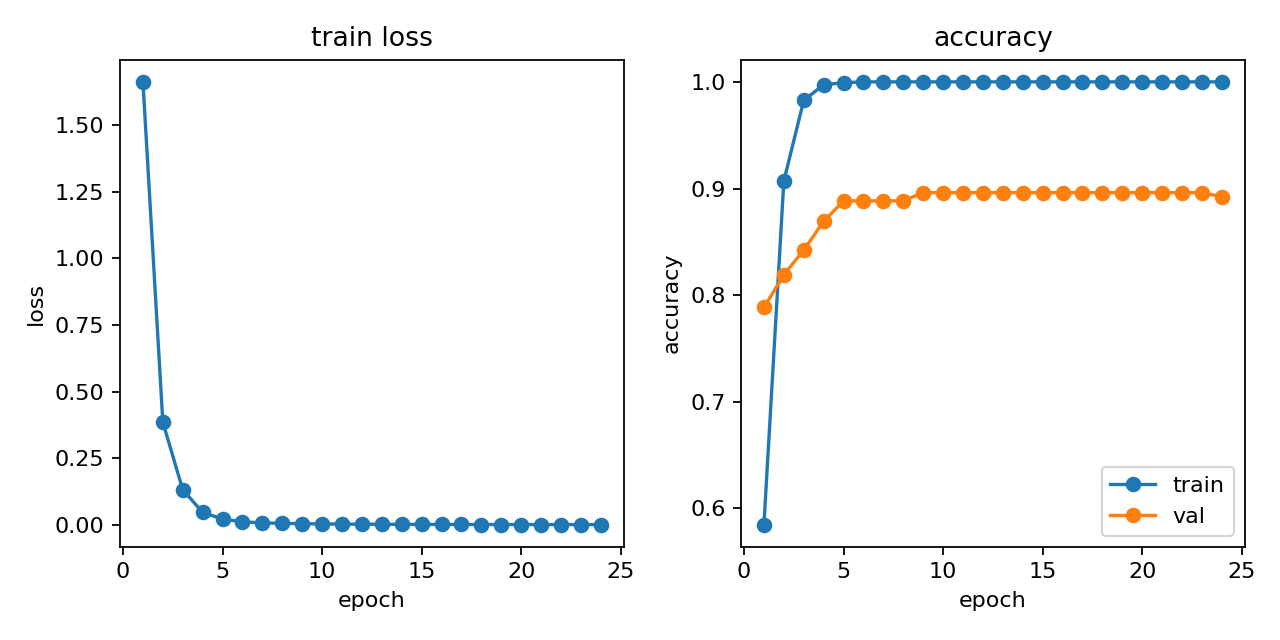
\includegraphics[width=0.82\linewidth]{figures/curve_mindcv_mobilenet_v2_100_lora_real.png}
  \caption{MindCV MobileNetV2-1.0 LoRA 微调曲线}
  \label{fig:mobile_lora}
\end{figure}

\subsection{MobileNetV2 中 LoRA 的意义}

LeNet5 上的 LoRA 边际收益有限，因为模型本身只有约 6.3 万参数。MobileNetV2 上的 LoRA 更能体现参数高效微调的意义：MindCV MobileNetV2-1.0 LoRA 只训练约 8.1 万参数，准确率达到 89.62\%，接近全量 cosine 微调的 91.15\%，同时训练时间为 459.41 s，低于全量 cosine 的 622.66 s。

在该实验中，LoRA 主要插入到 MobileNetV2 后部的 $1\times1$ pointwise convolution 层。这些层负责通道混合和高层语义特征调整，适合用低秩分支进行轻量适配。设原卷积或线性映射的权重更新为 $\Delta W$，LoRA 用两个低秩矩阵近似该更新，即 $\Delta W=BA\cdot\alpha/r$，从而避免直接训练完整权重矩阵。对于 MobileNetV2 这类参数量百万级的网络，LoRA 可以明显减少可训练参数量，并降低优化时需要保存的梯度和优化器状态。

这也解释了 LeNet5 与 MobileNetV2 中 LoRA 表现的差异。LeNet5 参数太少，全量微调本身成本已经很低，LoRA 的节省空间有限；而 MobileNetV2 参数规模更大，且预训练特征更强，冻结主干后只给中后层增加低秩可训练分支，就能在较低训练成本下接近全量微调精度。因此，LeNet5 中的 LoRA 更偏向方法实现验证，MobileNetV2 中的 LoRA 更能体现参数高效微调的实际价值。

\subsection{MobileNetV2-0.75 宽度版本实验}

为了进一步观察模型宽度对迁移学习效果的影响，本文还测试了 MindCV MobileNetV2-0.75。该模型将通道宽度缩小，总参数约 141 万，低于 MobileNetV2-1.0 的约 229 万。结果如\cref{tab:mobile_075} 所示。

\begin{table}[!htb]
  \centering
  \caption{MindCV MobileNetV2-0.75 补充实验结果}
  \label{tab:mobile_075}
  \small
  \begin{tabular}{@{}lrrrr@{}}
    \toprule
    \textbf{策略} & \textbf{可训练参数} & \textbf{时间} & \textbf{峰值显存} & \textbf{准确率} \\
    \midrule
    freeze & 33306 & 378.74 s & 3367 MB & 83.85\% \\
    full constant & 1415370 & 553.01 s & 4453 MB & 17.31\% \\
    full cosine & 1415370 & 576.85 s & 4453 MB & 90.77\% \\
    LoRA & 70298 & 395.93 s & 3429 MB & 87.69\% \\
    \bottomrule
  \end{tabular}
\end{table}

0.75 版本的结果与 1.0 版本总体一致：冻结和 LoRA 在完整预训练权重下表现稳定，全量微调必须配合学习率衰减；常量学习率全量微调明显不可靠。full cosine 达到 90.77\%，略低于 1.0 版本的 91.15\%，说明在该数据集规模下，缩小网络宽度只带来有限准确率损失。LoRA 达到 87.69\%，低于 1.0 版本 LoRA 的 89.62\%，但仍明显高于 LeNet5 和自实现 MobileNetV2，说明高质量预训练权重比单纯增加或减少网络宽度更关键。

从资源消耗看，0.75 版本 full cosine 的峰值显存为 4453 MB，高于 freeze 和 LoRA 的 3367 MB、3429 MB。LoRA 在保持较高准确率的同时，显存更接近冻结微调，这与参数高效微调的设计目标一致。该结果也补充说明：当模型规模增大后，冻结、LoRA、全量微调在资源占用上的差异会比 LeNet5 更明显。

\subsection{与 LeNet5 实验的互补关系}

MobileNetV2 进阶对照实验使本文结论更完整。LeNet5 适合完成课程设计中的基础迁移学习链路：先在 MNIST 上训练，再迁移到垃圾分类，并分别比较从零训练、冻结微调、全量微调和 LoRA 微调。由于 LeNet5 结构简单、层次清晰，冻结哪些层、训练哪些层、LoRA 加在哪些层都容易解释。

MobileNetV2 则从真实应用角度补充说明：如果目标是提高垃圾分类准确率，应尽量保留颜色信息、使用更高输入分辨率，并加载与模型结构匹配的高质量预训练权重。从结果看，LeNet5 全量微调 64.23\% 已经说明 MNIST 初始化具有一定价值，但模型受限明显；MindCV MobileNetV2-1.0 full + cosine 达到 91.15\%，说明垃圾分类任务本身并非不可学，而是 LeNet5 的输入适配和模型容量限制了上限。

因此，两组实验并不是互相替代的关系。LeNet5 回答“迁移学习、冻结微调和 LoRA 如何在一个可控的小型 CNN 中实现”，MobileNetV2 回答“在更接近实际视觉任务的输入和预训练条件下，垃圾分类性能可以提升到什么程度”。前者保证实验机制清楚，后者使结果分析更贴近真实应用。

\chapter{总结与不足}\label{chap:conclusion}

\section{实验总结}

本文围绕手写数字识别与垃圾分类两个任务完成了完整的深度学习课程设计。实验首先在 MNIST 上训练 LeNet5，取得 98.60\% 的测试准确率，并保存预训练权重；随后将该权重迁移到 26 类垃圾分类任务，完成从零训练、冻结微调、全量微调、LoRA 微调和强数据增强改进实验。

实验结果表明，垃圾分类从零训练效果很差，仅 3.85\%，说明小规模真实图片数据难以支撑 LeNet5 从随机初始化中直接学习。冻结微调只训练最后分类层，准确率为 15.38\%，说明 MNIST 预训练权重有一定迁移价值，但冻结主干限制了新任务适配能力。LoRA 微调在 \texttt{fc1} 和 \texttt{fc2} 上加入低秩分支，可训练参数为 5106，准确率达到 25.38\%，高于冻结微调。全量微调开放全部参数，准确率达到 64.23\%，是本实验中表现最好的策略。

强数据增强改进实验未能提升性能，准确率从 64.23\% 降至 38.85\%。通过预处理可视化可以看到，随机旋转在 $32\times32$ 灰度图上引入了明显黑色边框，可能形成无关伪特征。因此该实验的主要结论不是“数据增强无效”，而是当前增强算子配置存在改进空间，后续应检查填充值、插值方式和增强顺序。

MobileNetV2 进阶对照实验进一步说明，LeNet5 的局限主要来自输入适配和模型容量，而不是训练流程本身。使用 MindCV 官方预训练 MobileNetV2-1.0、RGB 输入和 $224\times224$ 分辨率后，冻结微调达到 87.31\%，LoRA 达到 89.62\%，全量微调配合 warmup + cosine 学习率衰减达到 91.15\%。这为垃圾分类任务提供了更接近真实应用场景的性能参照。

\section{LeNet5 在垃圾分类上的局限}

LeNet5 能够清晰展示卷积神经网络和迁移学习的基本流程，但在垃圾分类任务上存在明显局限：

\begin{enumerate}[label=(\arabic*)]
  \item \textbf{颜色信息丢失}：垃圾分类图片由 RGB 转为灰度，颜色线索被丢弃，而颜色常常是区分塑料、金属、纸张、果皮等类别的重要依据；
  \item \textbf{输入尺寸过小}：$32\times32$ 输入会压缩真实物体的纹理和局部细节，不利于细粒度分类；
  \item \textbf{模型容量有限}：LeNet5 层数浅、参数少，对 26 类真实场景图片的表达能力不足；
  \item \textbf{源任务与目标任务差异大}：MNIST 是简单手写数字，垃圾分类是真实物体图片，二者分布差异大，因此冻结主干迁移效果有限；
  \item \textbf{LoRA 边际收益有限}：LeNet5 本身参数很少，使用 LoRA 不会像大模型微调那样显著节省显存或训练时间，其主要价值是教学性和实现验证。
\end{enumerate}

\section{后续改进方向}

后续可以从以下方向改进：

\begin{enumerate}[label=(\arabic*)]
  \item 使用三通道颜色输入，设计三通道 LeNet 变体，减少颜色信息损失；
  \item 适当增大输入分辨率，例如 $64\times64$ 或 $96\times96$，保存更多纹理细节；
  \item 在 LeNet5 中加入 Dropout、BatchNorm 或更合理的数据增强策略，控制过拟合；
  \item 修正强数据增强的旋转填充值和插值配置，避免在低分辨率灰度图上产生黑色边框伪特征；
  \item 绘制混淆矩阵，分析易混类别并设计针对性增强；
  \item 继续测试 MobileNetV2、ResNet 等更强模型，与 LeNet5 实验形成多尺度对照。
\end{enumerate}

总体而言，本实验完成了从 MNIST 预训练到垃圾分类微调的完整 LeNet5 流程，并通过冻结、全量、LoRA 和数据增强实验展示了不同训练策略在准确率、可训练参数量、训练时间和显存占用上的差异。


\makereferences

\appendix
\chapter{关键运行命令}\label{app:commands}

\section{一键运行 LeNet5 实验}

在项目根目录下运行：

\begin{lstlisting}[language=bash,numbers=none]
powershell -ExecutionPolicy Bypass -File scripts/run_lenet_experiments.ps1
\end{lstlisting}

该脚本依次运行 MNIST 预训练、垃圾分类从零训练、冻结微调、全量微调、LoRA 微调和强数据增强改进实验，并绘制所有训练曲线。

\section{分步命令}

\begin{lstlisting}[language=bash,numbers=none]
# MNIST 预训练
docker compose run --rm mindspore-gpu python src/train_mnist_lenet.py \
  --run_name lenet_mnist --epochs 5 --batch_size 64 \
  --image_size 32 --lr 1e-3

# 垃圾分类从零训练
docker compose run --rm mindspore-gpu python src/train_lenet_garbage.py \
  --data_dir data/garbage_official --mode scratch \
  --run_name lenet_garbage_scratch --epochs 24 \
  --batch_size 32 --image_size 32 --lr 1e-3 --weight_decay 1e-4

# 冻结微调
docker compose run --rm mindspore-gpu python src/train_lenet_garbage.py \
  --data_dir data/garbage_official \
  --pretrained checkpoints/lenet_mnist.ckpt \
  --mode freeze --run_name lenet_garbage_freeze \
  --epochs 24 --batch_size 32 --image_size 32 \
  --lr 1e-3 --weight_decay 1e-4

# 全量微调
docker compose run --rm mindspore-gpu python src/train_lenet_garbage.py \
  --data_dir data/garbage_official \
  --pretrained checkpoints/lenet_mnist.ckpt \
  --mode full --run_name lenet_garbage_full \
  --epochs 24 --batch_size 32 --image_size 32 \
  --lr 1e-3 --weight_decay 1e-4

# LoRA 微调
docker compose run --rm mindspore-gpu python src/train_lenet_garbage.py \
  --data_dir data/garbage_official \
  --pretrained checkpoints/lenet_mnist.ckpt \
  --mode lora --run_name lenet_garbage_lora \
  --epochs 24 --batch_size 32 --image_size 32 \
  --lr 1e-3 --weight_decay 1e-4 --lora_rank 4 --lora_alpha 8

# 强数据增强改进实验
docker compose run --rm mindspore-gpu python src/train_lenet_garbage.py \
  --data_dir data/garbage_official \
  --pretrained checkpoints/lenet_mnist.ckpt \
  --mode full --run_name lenet_garbage_full_aug \
  --epochs 24 --batch_size 32 --image_size 32 \
  --lr 1e-3 --weight_decay 1e-4 --strong_aug
\end{lstlisting}

\section{评估与曲线绘制}

\begin{lstlisting}[language=bash,numbers=none]
docker compose run --rm mindspore-gpu python src/eval_lenet.py \
  --data_dir data/garbage_official \
  --ckpt checkpoints/best_lenet_garbage_full.ckpt \
  --num_classes 26 --out results/eval_lenet_garbage_full.json

docker compose run --rm mindspore-gpu python src/plot_curves.py \
  --log logs/train_lenet_garbage_full.csv \
  --out results/curve_lenet_garbage_full.png
\end{lstlisting}

\chapter{MobileNetV2 进阶对照命令示例}

正文第 \ref{chap:experiment} 章已经给出 MobileNetV2 进阶对照实验的核心结果。这里列出对应运行命令，便于复现。

\begin{lstlisting}[language=bash,numbers=none]
# MindCV MobileNetV2-1.0 full + cosine
docker compose run --rm mindspore-gpu python src/train_official_mobilenet.py \
  --data_dir data/garbage_official \
  --model_name mobilenet_v2_100_224 \
  --checkpoint_path checkpoints/mindcv_mobilenet_v2_100.ckpt \
  --mode full --epochs 24 --batch_size 16 --lr 1e-4 \
  --lr_schedule cosine --min_lr 1e-6 --warmup_epochs 2

# MindCV MobileNetV2-1.0 LoRA
docker compose run --rm mindspore-gpu python src/train_official_mobilenet.py \
  --data_dir data/garbage_official \
  --model_name mobilenet_v2_100_224 \
  --checkpoint_path checkpoints/mindcv_mobilenet_v2_100.ckpt \
  --mode lora --epochs 24 --batch_size 16 --lr 1e-3 \
  --lora_rank 4 --lora_alpha 8 --lora_max_layers 12
\end{lstlisting}


\end{document}
